\chapter{Acquisizione e analisi di dati da SiPM}

\section*{Obiettivi}
L'obiettivo di questo esperimento finale è di acquisire le onde generate da un SiPM con il nostro microcontrollore, comunicare i dati a MATLAB e fare un istogramma per visualizzare quanti fotoni vengono rilevati.

\section*{Scheda SiPM}

\begin{figure}[H]
\centering
\includegraphics[width=\textwidth]{assets/exp9/scheda.png}
\caption{Scheda con SiPM e amplificatori}
\end{figure}

Sulla scheda troviamo innanzitutto il SiPM. Il SiPM è un dispositivo formato da più SPAD, dei diodi fotorilevatori a singolo fotone. Il modello di SiPM usato in questo esperimento è S13360-1350CS.
Questo sensore è sensibile ai fotoni, e genera una corrente proporzionale al numero di fotoni rilevati.


Al SiPM applichiamo una tensione in inversa Vop, il cui valore è una caratteristica del singolo SiPM. Come riportato in figura questa tensione è 54.2V.

\begin{figure}[H]
\centering
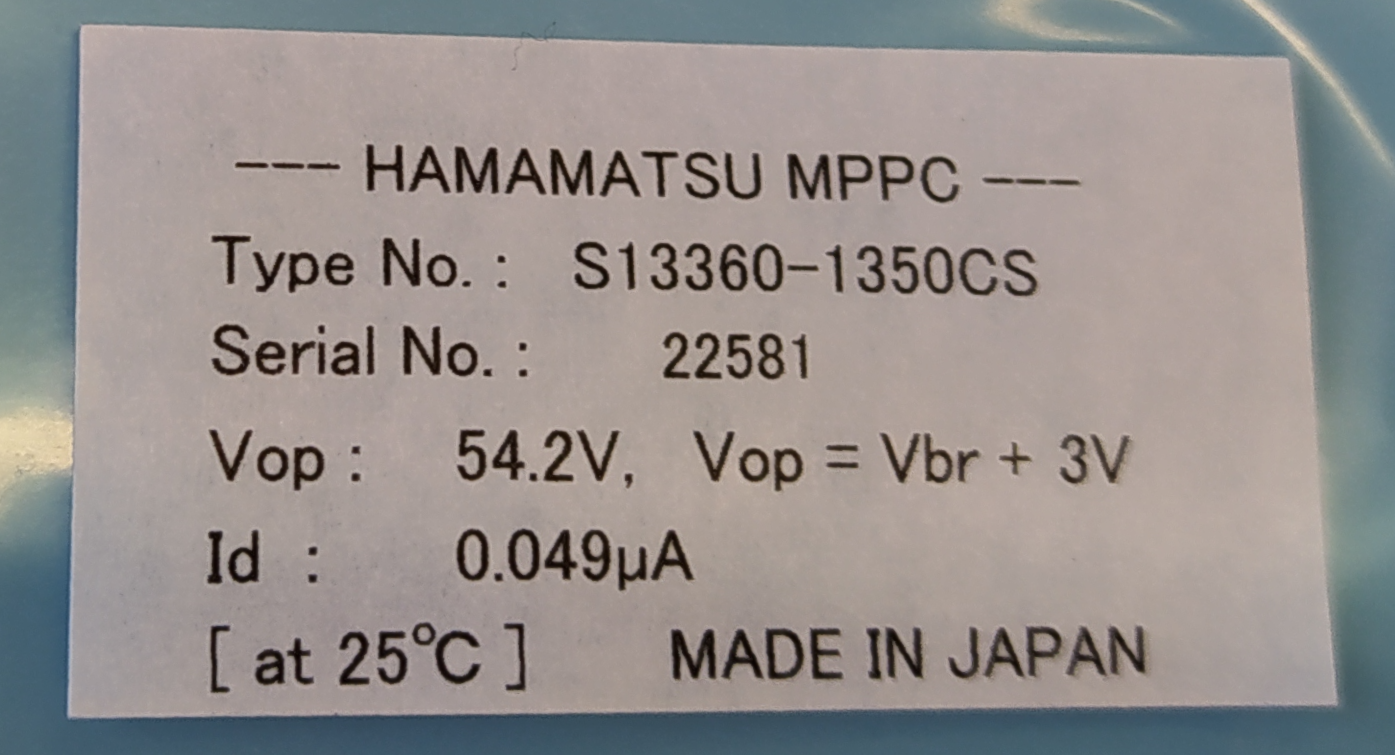
\includegraphics[width=0.5\textwidth]{assets/exp9/SiPM.png}
\caption{SiPM utilizzato}
\end{figure}

Vicino al SiPM troviamo un LED: useremo il generatore di funzioni per applicare una differenza di potenziale ai capi del LED, facendolo quindi illuminare.
Andiamo poi a coprire SiPM e LED con un coperchio, per permettere al SiPM di rilevare unicamente i fotoni provenienti dal LED.

Prima di poter acquisire il segnale con il nostro microcontrollore è necessario amplificarlo e sagomarlo in modo opportuno.

Il segnale generato dal SiPM è un segnale in corrente, mentre l'ADC presente sulla nostra scheda è in grado di effettuare una conversione in tensione.
Per questo motivo utilizziamo nel primo stadio un amplificatore operazionale in modalità invertente per convertire la corrente in tensione.

\begin{figure}[H]
\centering
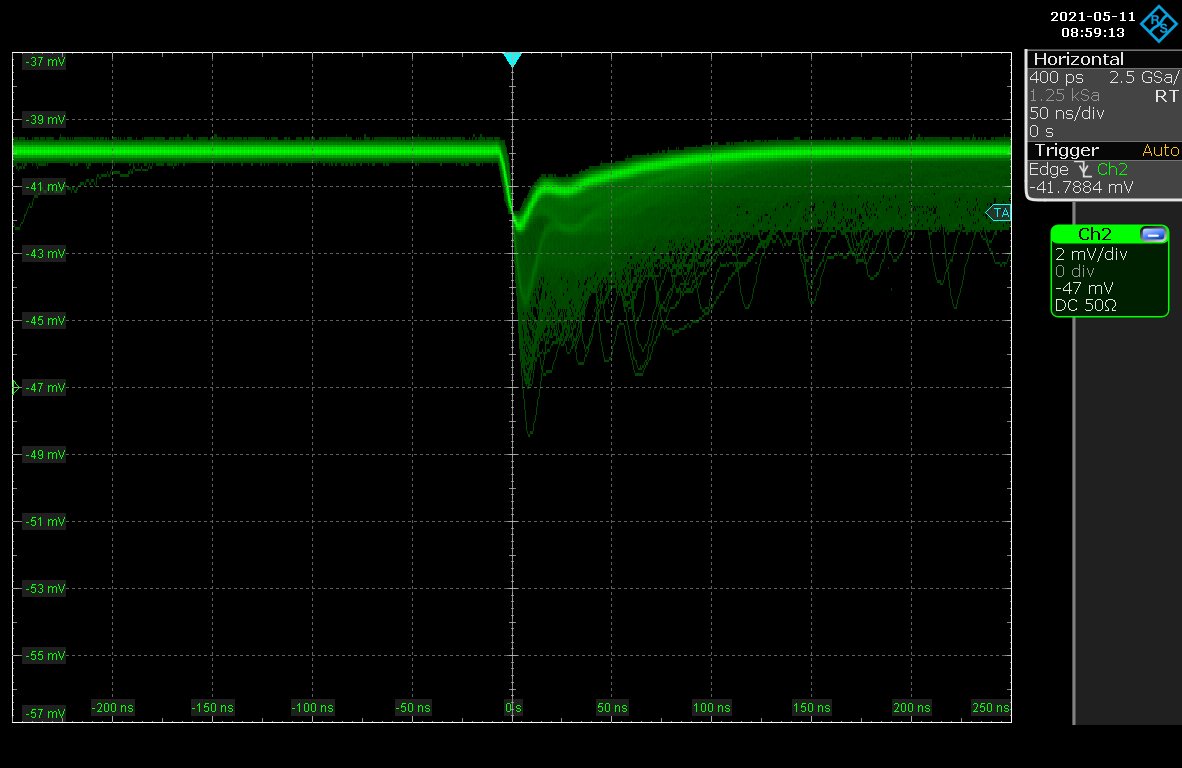
\includegraphics[width=0.7\textwidth]{assets/exp9/primo_stadio.png}
\caption{Segnale in uscita dal primo stadio}
\end{figure}

Notiamo quindi che il segnale in uscita dal primo stadio è un segnale la cui tensione è negativa.
Il nostro microcontrollore è in grado di convertire soltanto tensioni che variano tra 0 e 3.3V.
Andiamo quindi, nel secondo stadio, ad utilizzare un opamp AD9631 in modalità invertente per portare il segnale in positivo. Impostiamo un gain di circa 42, per avere una maggiore risoluzione, seguendo la seguente formula:

\begin{displaymath}
V_o = \frac{-RF}{R1} V_s \approx 42.3
\end{displaymath}

Troviamo quindi  $RF = 11 \si{\kilo\ohm}$ e $ R1 = 260 \si{\ohm}$

Come ultima fase abbiamo un circuito Peak and Hold: il segnale generato dal SiPM dura pochi nanosecondi e non saremmo quindi in grado di andarlo a campionare con il microcontrollore, in quanto è in grado di campionare a poco più di un MegaHertz. Dopo la fase di Peak and Hold ottieniamo un segnale più smussato e con un periodo più lungo, che siamo in grado di rilevare con l'ADC.

\begin{figure}[H]
\centering
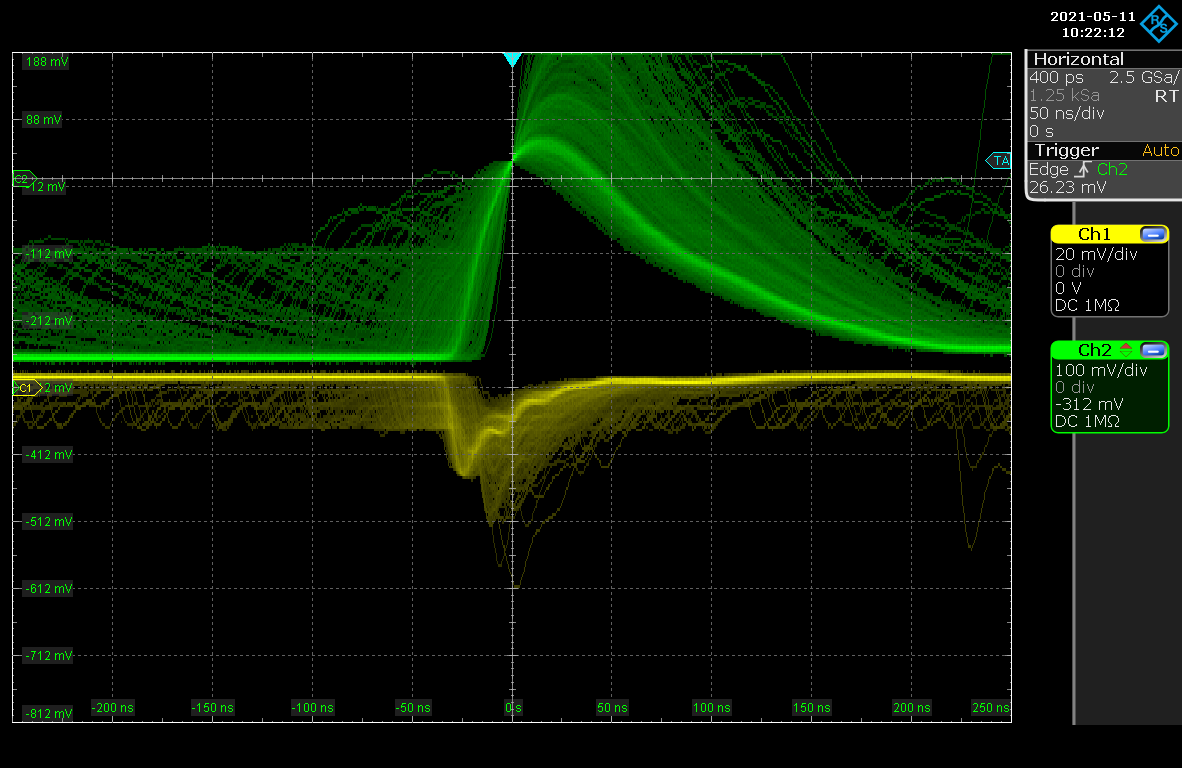
\includegraphics[width=0.7\textwidth]{assets/exp9/inv_g_42.png}
\caption{Segnale in uscita dal PH: in giallo l'output del primo stadio, in verde l'output del PH}
\end{figure}

Notiamo però che è rimasto un offset negativo anche al segnale finale: per questo motivo è stata aggiunta nel secondo stadio una resistenza per iniettare una corrente positiva e avere un offset positivo, sempre per poter acquisire il segnale con il microcontrollore.

Tutte le fasi precedenti sono state testate soltanto andando a guardare i "dark counts" generati dal rumore termico, senza far illuminare il LED.

Andiamo quindi infine a generare un'onda con il generatore di funzioni per far illuminare il LED per una frazione di secondo. Il segnale di default è "alto", in questo modo non abbiamo caduta di tensione sul LED, e ogni 2ms viene generato un impulso che dura 200ns in cui il sengale è "basso": in questi 200ns modo abbiamo una caduta di tensione sul LED che quindi si illumina.

Possiamo poi andare ad analizzare con l'oscilloscopio, acquisendo più volte le onde, il numero di fotoni rilevati dal SiPM. Ricordando che il SiPM genera una corrente proporzionale al numero di fotoni rilevati, possiamo visualizzare un istogramma sull'ampiezza del segnale rilevato: i picchi nell'istogramma corrispondono al numero di fotoni rilevati.

\begin{figure}[H]
\centering
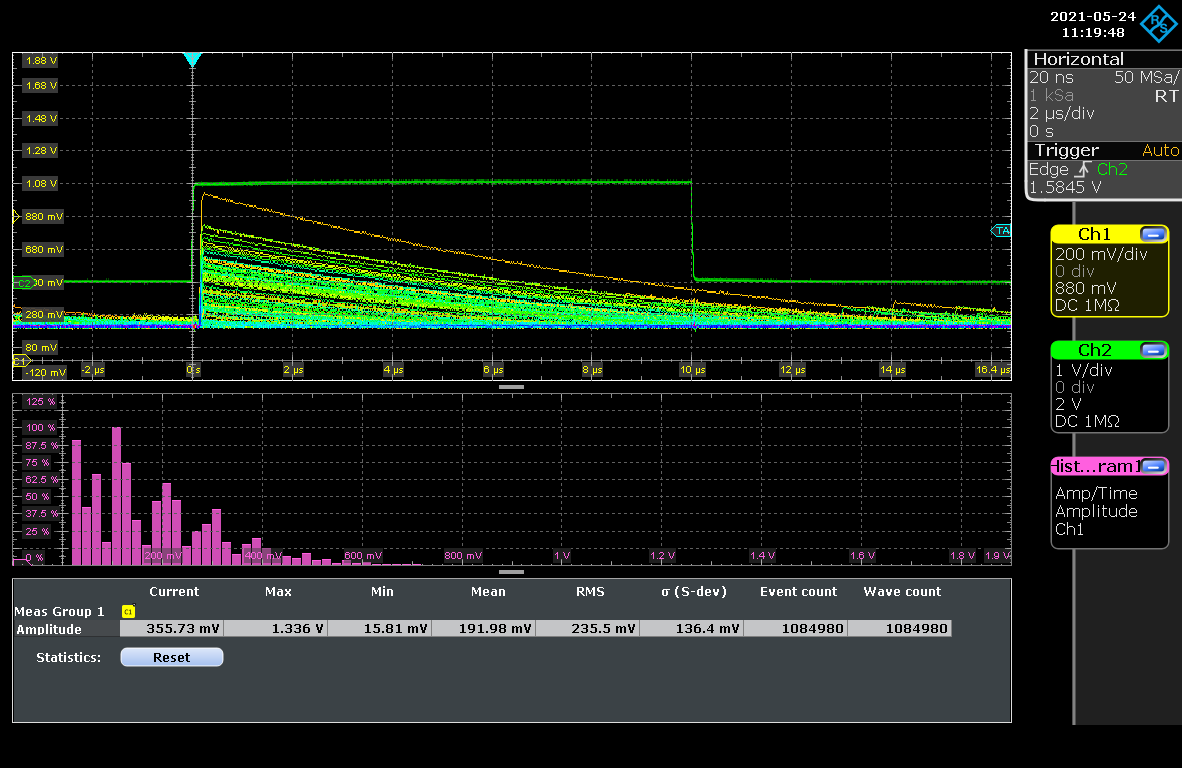
\includegraphics[width=\textwidth]{assets/exp9/sipm_oscilloscopio_istogramma.png}
\caption{Onde generate dal SiPM dopo lo stadio di PH e facendo illuminare il LED, con relativo istogramma}
\end{figure}

\section*{MATLAB}
Per fare un'analisi statistica dei dati come quella fatta dall'oscilloscopio è necessario acquisire più campioni di fila.
È stato quindi utilizzato il seguente codice MATLAB per richiedere al microcontrollore di acquisire i campioni per un numero arbitrario di volte. Ad ogni acqusizione salviamo il massimo valore ricevuto, e alla fine delle acquisizioni andiamo a fare un istogramma dei picchi rilevati.


\begin{minted}
[
frame=lines,
framesep=2mm,
baselinestretch=1.2,
fontsize=\footnotesize,
]{MATLAB}
data = [];

for i = 1:1000
    new_data = testUART(201, 'uint16');
    data = [data max(new_data(1:200))];
    disp(i);
end

histogram(data,100)
\end{minted}

\section*{Acquisizione microcontrollore con trigger su ADC}
Come prima cosa abbiamo provato ad acquisire il segnale del SiPM utilizzando un trigger sul valore di ADC, come visto nell'esperimento \ref{chap:adc_trigger}.


\begin{figure}[H]
\centering
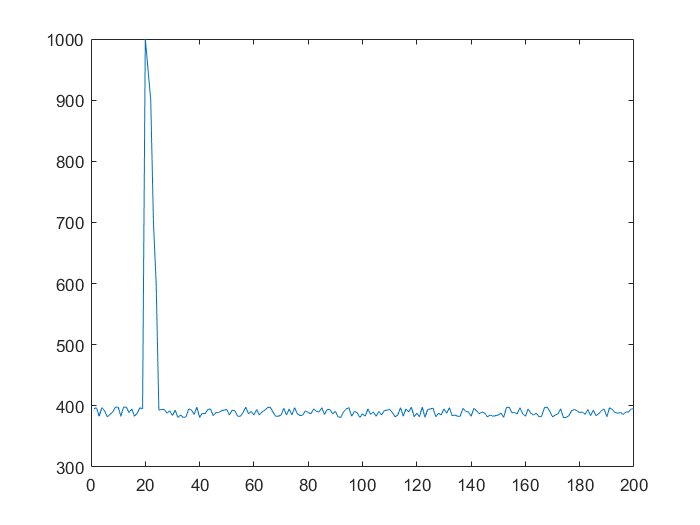
\includegraphics[width=0.6\textwidth]{assets/exp9/matlab_peak.png}
\caption{Plot di una singola onda rilevata}
\end{figure}

\begin{figure}[H]
\centering
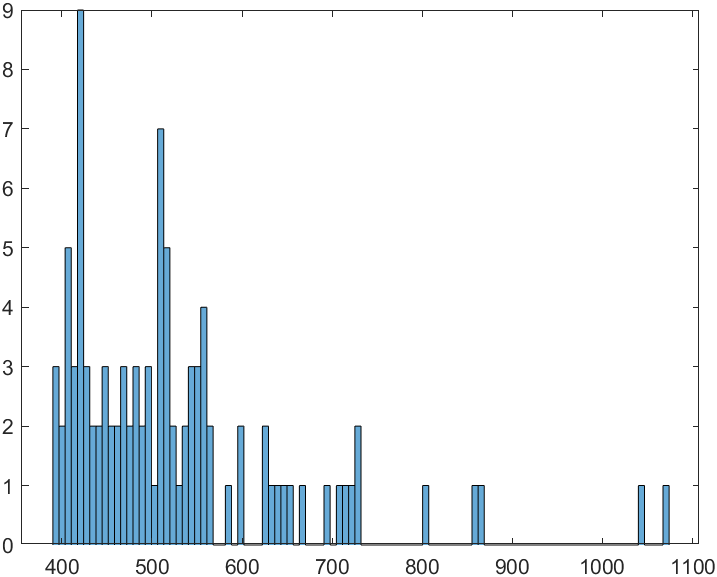
\includegraphics[width=0.6\textwidth]{assets/exp9/hist_matlab_2.png}
\caption{Istogramma utilizzando il trigger sull'ADC}
\end{figure}


\section*{Acquisizione microcontrollore con trigger su ingresso digitale}
Come ultima prova abbiamo acquisito i segnali sfruttando un trigger digitale al posto di quello sull'ADC \footnote{\href{https://github.com/fdila/electronics-experimentation/tree/main/Exp10}{Il codice è disponibile nella repository, cartella Exp10}}. 

Come prima dobbiamo generare il segnale di trigger con il generatore di funzioni: il segnale che usiamo per far illuminare il LED resta uguale, e generiamo poi un segnale che di default è basso e che, sincronizzato al primo segnale, diventa alto per 10 microsecondi. Colleghiamo questo nuovo segnale generato ad un pin del microcontrollore.

Tramite CubeMX andiamo a configurare il pin a cui abbiamo collegato il segnale come EXTI, ovvero andiamo a generare un interrupt quando viene rilevato un fronte di salita sul pin.

Nella routine di interrput dell'EXTI accendiamo un flag. Ad ogni conversione dell'ADC, nella sua routine di interrupt, andiamo a controllare questo flag: se è stato rilevato un fronte di salita, quindi abbiamo fatto illuminare il LED, teniamo l'indice corrente a cui ci troviamo nel buffer come indice del picco. Acquisiamo quindi i restanti campioni come nell'esperimento \ref{chap:adc_trigger} e inviamo i dati raccolti a MATLAB.


\begin{figure}[H]
\centering
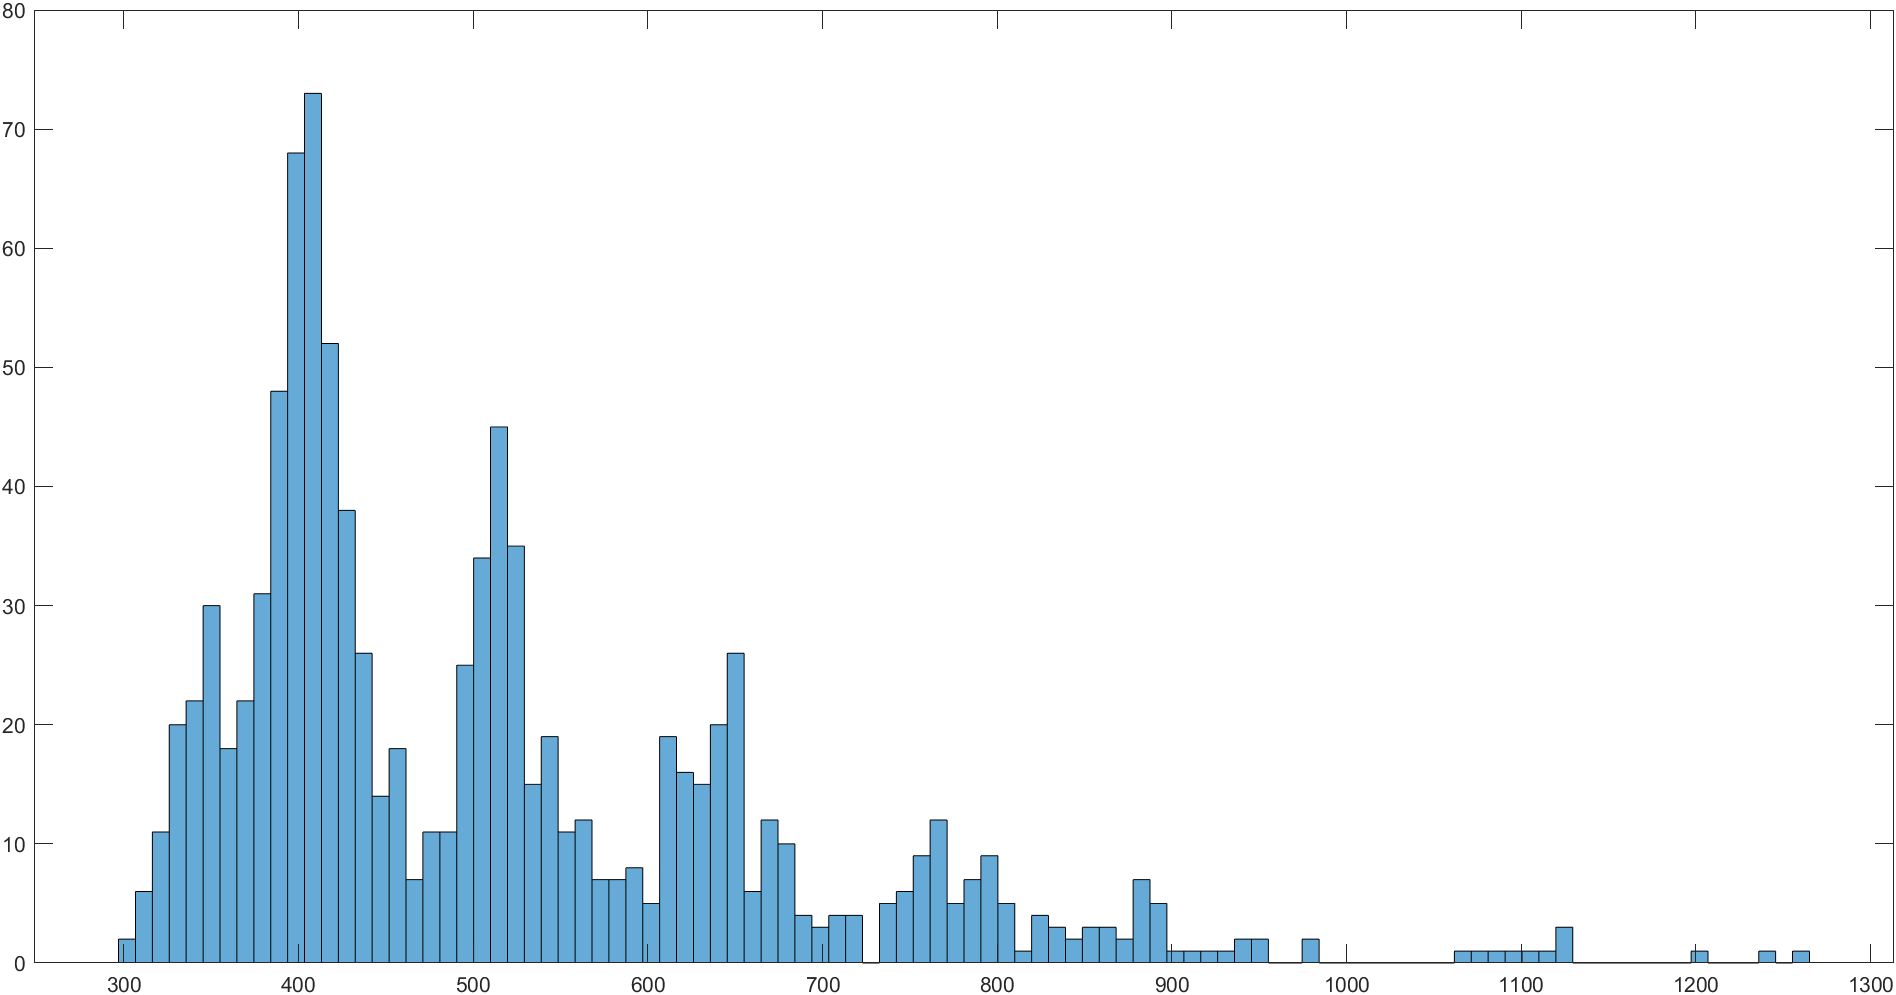
\includegraphics[width=\textwidth]{assets/exp9/hist_matlab_5.png}
\caption{Istogramma utilizzando il trigger sull'impulso del generatore di funzioni}
\end{figure}